\section{Descripción general de las pruebas}
La población total sobre la cual se realizó el estudio es de 2388 individuos
distribuídos en 85 puntos de control. Cada punto control tiene entre 0 y 133
individuos en el estado larval con edad 0; todas las larvas tienen la misma edad
en el instante inicial de las pruebas.Además, los individuos comparten
las mismas condiciones climáticas, es decir, la temperatura es la misma
para todos los puntos de control \\

\begin{figure}
\centering
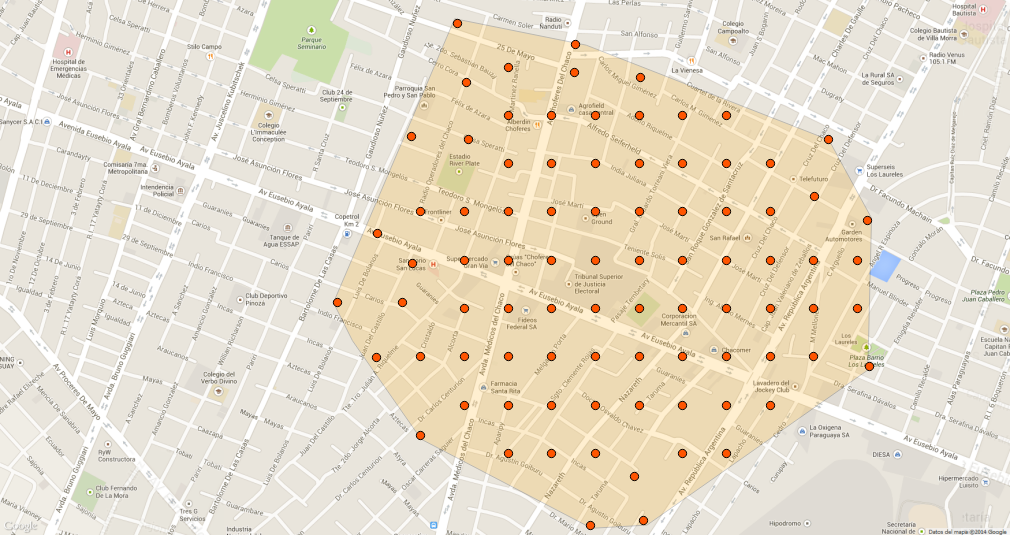
\includegraphics[width=0.9\textwidth]{./capitulo-6/graphics/puntoscontroldistribuido.png}
\caption{\label{fig:distribucion-puntos}Ubicación geográfica y distribución de puntos de control.}
\end{figure}


En la \figref{fig:distribucion-puntos} se observa la distribución de los puntos de control.
Geográficamente corresponde a 4 barrios de la ciudad de Asunción, Paraguay. Los barrios son
Nazareth, Terminal, San Pablo e Hipódromo. Es importante aclarar que la ubicación geográfica
exacta no es relevante para el desarrollo de las pruebas, ya que no se utilizaron
condiciones climáticas propias de dicha ubicación. La ubicación geográfica sirve
de referencia y para poder georeferenciar resultados finales. El área de covertura
es de 2.9$km^2$ y los puntos de control se hallan ubicados uniformemente distribuidos.\\


\begin{table}
    \begin{center}
        \caption{ \label{tab:valores-formulas} Valores de parámetros en fórmulas utilizadas}
        \begin{tabular}{p{3cm} c c c c}
            \hline \\
            Variable & Simbolo & Valor & Fórmula \\
            \hline
            \hline \\
            Sitios de reproducción &  BS & 50 & ver fórmula xxx\\
            Inhibición de eclosión de huevos & $A_{0}$ & 0.5 & ver fórmula xxx\\
        \end{tabular}
    \end{center}
\end{table}

La duración total de días en cada prueba es 50, se toma como día 0 el instante
inicial del proceso evolutivo y como día final al día 49. Para observar la variación
de propiedades biológicas del mosquito Aedes Aegypti se realizaron pruebas a distintas
temperaturas, dichas temperaturas se mantienen constantes durante cada prueba y son las siguientes :
15\textcelsius , 18\textcelsius , 20\textcelsius , 22\textcelsius ,
24\textcelsius , 25\textcelsius , 26\textcelsius , 27\textcelsius ,
30\textcelsius , 34\textcelsius \\


Se realizaron N iteraciones del algoritmo evolutivo y se realizaron las
validaciones sobre el conjunto de datos generado por el mismo

Se presentan los resultados para tasa de desarroollo de las etapas inmaduras
(HUEVO, LARVA y PUPA) del Aedes Aegypti, mortalidad en cada una de las etapas,
la ovipostura, duracion del ciclo gonotrofico, alimentacion, promedio de vuelo y
desplazamiento y distribucion de sexos


